\chapter{Theoretical background}
\section{Complex networks and their properties}
A \textbf{graph} (network) $\mathcal{G}$ is a set of \textbf{vertices} (nodes) $V$ and a set of \textbf{edges} (links) $E$ connecting the vertices. Vertices are distinguishable, so we can explicitly label them $i = 1,\dots,N$ where $N$ is the number of vertices. Then we can define the \textbf{adjacency matrix} $\mathbb{A}$, whose entries are
\begin{equation*}
a_{ij} = \begin{cases}
1 \text{ if there is an edge from node \textit{i} to \textit{j}} \\
0 \text{ otherwise}
\end{cases}
\end{equation*}
Graphs can be \textbf{directed} or \textbf{undirected}. In the undirected case, $a_{ij} = a_{ji}$, i.e., the adjacency matrix is symmetric, directed graphs do not have such a constraint.
A graph can be \textbf{weighted}. This means that each edge present in the graph can be assigned a weight, a real number $w_{ij}$.
\subsection{Network properties}
When studying networks, we are usually interested in their properties, which can give us an idea about their topology. Let us mention a few of them.
\subsubsection{Degrees}
\textbf{Degree} of a node corresponds to the number of its neighbors, i.e., the number of edges adjacent to it. In a directed graph, we need to distinguish between \textbf{in-degree} and \textbf{out-degree}. Using the adjacency matrix, they can be written in a simple way,
\begin{align}
k_i^{in} &= \sum_{i=1}^{N} a_{ji} \\
k_i^{out} &= \sum_{i=1}^{N} a_{ij}
\end{align}
In an undirected graph, there is only the total degree of each node,
\begin{equation}
k_i = \sum_{i=1}^{N} a_{ij}
\end{equation}
To obtain some useful information about the whole graph, we can study the \textbf{degree distribution}. The degree distribution $P(k)$ denotes the fraction of nodes in the graph with degree $k$. It has been shown that large number of real-world networks have a power-law degree distribution $P(k) \sim k^{-\gamma}$ \cite{Barabasi1999}. These networks are usually called \textbf{scale-free}.
\subsubsection{Strengths}
On weighted networks, we can also define the node \textbf{strength}. The strength of a node is the sum of all weights of its adjacent edges. Similarly to degrees, we define in-strength and out-strength on a directed graph,
\begin{align}
s_i^{in} &= \sum_{i=1}^{N} w_{ji} \\
s_i^{out} &= \sum_{i=1}^{N} w_{ij}
\end{align}
or just a single strength on an undirected graph. Similarly to degrees, strengths also often exhibit a power-law structure \cite{Yook2001}.
\subsubsection{Average nearest neighbor degree}
Now we move on to the second-order properties. For these properties, we do not only take into account the neighbors of a node, but also neighbors of neighbors. The first example of such a property is the \textbf{average nearest neighbor degree} (ANND). It can be defined for in-going and out-going links. We define the average out-degree of out-neighbors of node $i$ as
\begin{equation}
k_{i}^{nn,out} = \frac{\sum_{j\neq i}a_{ij} k_j}{k_i} = \frac{\sum_{j\neq i}\sum_{k\neq j}a_{ij} a_{jk}}{\sum_{j\neq i}a_{ij}}
\end{equation}
The average in-degree of in-neighbors of node $i$ is
\begin{equation}
k_{i}^{nn,in} = \frac{\sum_{j\neq i}\sum_{k\neq j}a_{ji} a_{kj}}{\sum_{j\neq i}a_{ji}}
\end{equation}
We could also define the average out-degree of in-neighbors and vice versa, but we will not use these.
One property of interest in real-world networks can be their \textbf{assortativity}. Assortativity means the tendency of nodes with certain features to be neighbors with nodes of similar features. In the context of node degrees, we can study \textit{assortativity by degree}, i.e. whether nodes with high degrees are usually connected to nodes with high degrees or not. If the ANND increases with the degree of a node, we call the network \textbf{assortative}; if the ANND decreases, we call it \textbf{disassortative}.

\subsubsection{Average nearest neighbor strength}
Similarly to the average nearest neighbor degree, we can define the \textbf{average nearest neighbor strengths} as
\begin{align}
s_{i}^{nn,out} &= \frac{\sum_{j\neq i}\sum_{k\neq j}a_{ij} w_{jk}}{\sum_{j\neq i}a_{ij}} \\
s_{i}^{nn,in} &= \frac{\sum_{j\neq i}\sum_{k\neq j}a_{ji} w_{kj}}{\sum_{j\neq i}a_{ji}}
\end{align}

\subsubsection{Local clustering coefficient}
The local clustering coefficient is defined on an undirected projection of our graph, whose adjacency matrix can be obtained as
\begin{equation}
b_{ij} = \max(a_{ij}, a_{ji})
\end{equation}

The idea of the local clustering coefficient is to look at all neighbors of a selected node and find out, how many of all possible links between these neighbors are realized. If neighbors of a node are highly connected among each other, we assume such a node is in a group of highly connected nodes, which we call cluster. Mathematically, the local clustering coefficient of the $i$-th node can be expressed as
\begin{equation}
c_i = \frac{\sum_{j\neq i}\sum_{k\neq i,j}b_{ij} b_{jk} b_{ki}}{\sum_{j\neq i}\sum_{k\neq i,j}b_{ij}b_{ki}}
\end{equation}


\section{Random network models}
In this section, we will introduce the basic concepts of network modeling. Networks are usually modeled using stochastic models. Two approaches are usually taken \cite{Cimini2019}:
\begin{itemize}
    \item \textbf{Microscopic}: In these models, some microscopic network formation mechanism is identified and used to reproduce properties of real-world systems. Such models include, for example, the Barabási-Albert preferential attachment model and the Watts-Strogatz small-world model.
    \item \textbf{Macroscopic}: Here, macroscopic properties of networks of interest are identified, and based on these properties, one finds models which reproduce them on average, but otherwise stay maximally random. This approach is similar to that of statistical mechanics. The framework used here is called Exponential Random Graphs.
\end{itemize}
We introduce both concepts in the following paragraphs.
\subsection{Erdős-Rényi model}
The Erdős-Rényi model is the simplest case of a random graph model. Let us have $n$ vertices. Let us fix a probability $0 \leq p \leq 1$. Then each possible edge is realized with probability $p$ and not realized with probability $1-p$. Edges are drawn independently.
This model is usually not suitable for reproducing properties of real-world networks. Some examples to mention are:

\begin{itemize}
    \item Degree distribution: Edges are drawn independently and each of them is a Bernoulli variable, therefore the degree of a node is a binomial random variable, which in the large $N$ limit with $pN$ bounded converges to a Poisson distribution, which decreases faster than exponentially. On the other hand, real-world networks usually have fat-tailed, power-law degree distributions.
    \item Average nearest neighbor degree: The expected average number of neighbors of each node in the Erdős-Rényi model is $p(N-1)$. Therefore, even the average nearest neighbor degree of each node is $p(N-1)$, a constant independent of the degree of the node. However, real-world networks are usually assortative or disassortative.
    \item Local clustering coefficient: The expected local clustering coefficient in the Erdős-Rényi model is $p$ for each node, however in real-world networks, the local clustering coefficient is usually a decreasing function of the node degree.
\end{itemize}

\subsection{Barabási-Albert preferential attachment model}
Barabási and Albert were interested in explaining how the scale-free degree distributions can emerge in real-world networks. They came up with two important observations:

\begin{itemize}
    \item Growth: Real-world networks are usually not static, they grow with time.
    \item Preferential attachment: When a new node emerges, it is more likely to connect to nodes that already have many connections.
\end{itemize}

With these observations, they came up with the following model \cite{Barabasi1999}. They start with a few vertices, for example two vertices connected with an edge. Then, in each step, they add one node (implementing growth). This node then connects to the already existing nodes with a probability proportional to their degree, $p(i) = k_i/\sum k_i$ (preferential attachement). They were then able to show that such a model yields a power-law degree distribution with an exponent $\gamma = 3$. Generalizations allowing for a tunable scaling exponent were also found \cite{Hofstad2016}.

\begin{figure}[!ht]
\centering
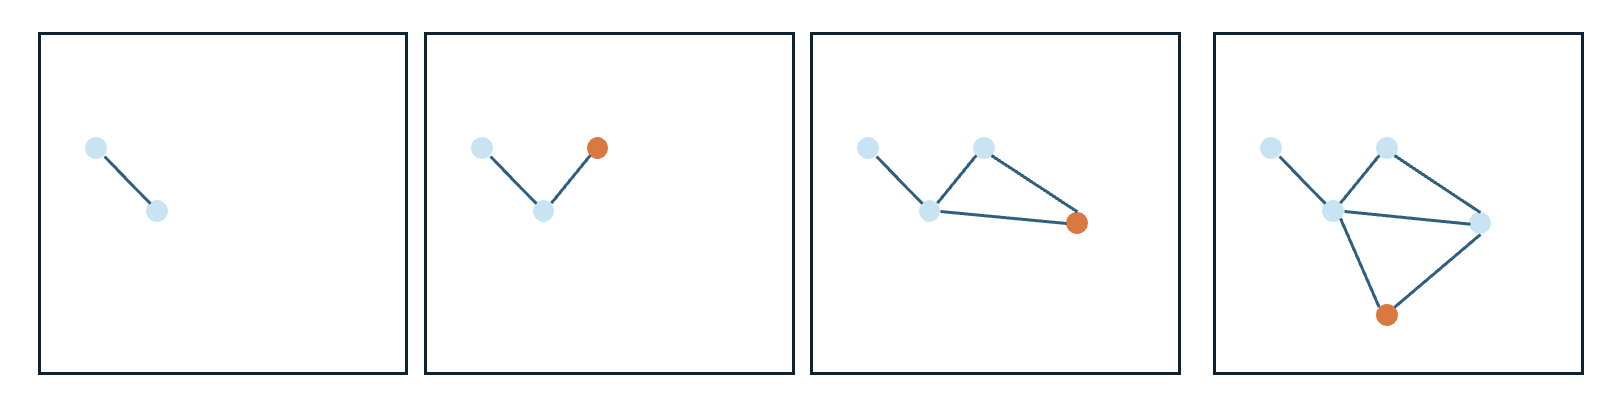
\includegraphics[scale=0.55]{../img/theory/preferential_attachement.png}
    \caption{Illustration of the Barabási-Albert model. Each step adds one node and connects it to other nodes with a probability proportional to their degree. In the figure, we can see that a new node tends to connect to nodes with an already high degree.}
    \label{fig:barabasi_albert}
\end{figure}

\subsection{Configuration model}
The configuration model starts with a prescribed degree sequence ${k_i}$ and tries to find graphs compatible with such that degree sequence. The simplest approach is to start with a desired number of vertices $N$ and assign to each node a number of half-edges that corresponds to its prescribed degree. These half-edges can be connected together to form full edges. One way to do that is to connect them uniformly randomly. That gives a random network model, which yields graphs with a degree sequence precisely corresponding to the prescribed one.

However, this version of the configuration model cannot avoid self-loops (edges going from some node to itself). Therefore, graphs generated by this model can usually hardly be compared with real-world networks. An approach avoiding this issue is called link stub reconnection. It starts with a real-world network without self-loops and reconnects its edges in such a manner that the degree sequence is preserved. However, this method was shown to explore the space of all allowed graphs non-uniformly, staying near the original graph. This can be overcome by introducing an acceptance-probability \cite{Coolen2009}, but that makes the whole problem more computationally demanding.

\begin{figure}[!ht]
    \centering
    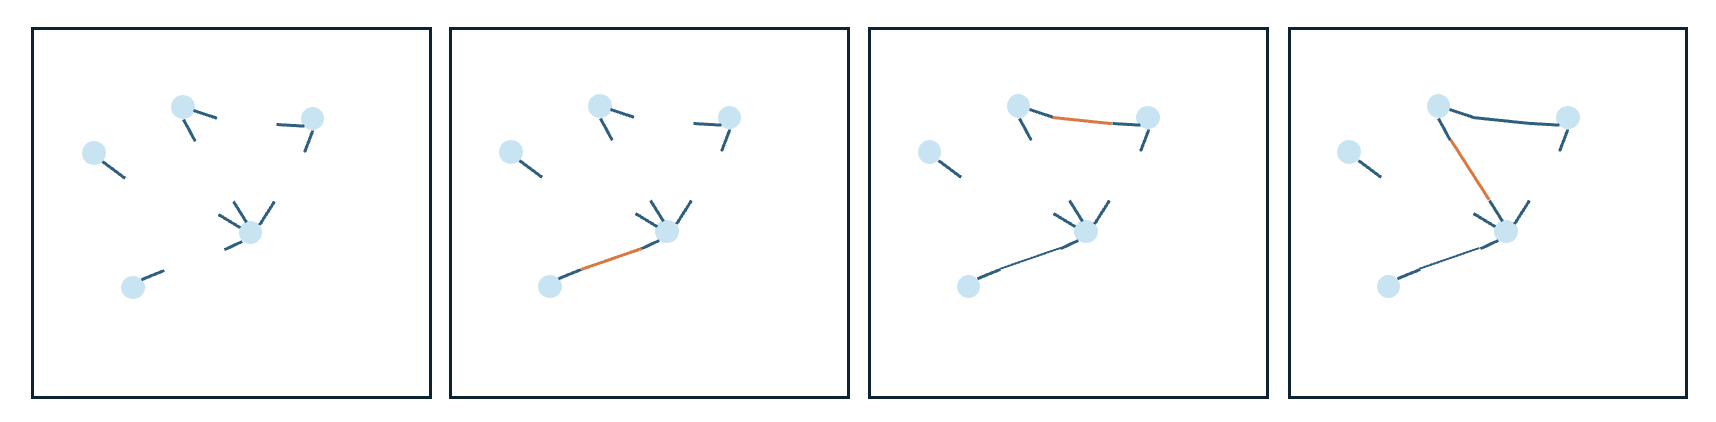
\includegraphics[scale=0.5]{../img/theory/configuration_model.png}
    \caption{Illustration of the configuration model. Each node possesses the so-called half-stubs or half-edges. The number of half-stubs corresponds to the desired degree. Then these half stubs are connected uniformly randomly to form full edges.}
    \label{fig:barabasi_albert}
\end{figure}

\subsection{Maximum-entropy ensembles of graphs}
\label{sec_max_ent_ensembles}
Random network models can not only produce a single realization, but a whole ensemble of graphs. Let us denote $\mathcal{G}$ all possible graphs (where we usually fix the number of nodes, we omit the notation here). Then a random network model essentially assigns a probability $P(G)$ to each graph $G \in \mathcal{G}$, s.t. $\sum_{G \in \mathcal{G}}P(G) = 1$. Let us recall the configuration model. This model was producing an ensemble of graphs with a fixed degree sequence. However, we also encountered several limitations. Essentially, the configuration model creates a microcanonical ensemble, constraint is forced in each realization. 

We can take another approach and only demand our constraints to be valid on average over the whole ensemble. To define a model, we need to assign probabilities to each graph possible. But from statistical physics, we know how to find the least biased probability distributions given constraints, using the maximum-entropy principle. This approach was used similarly for networks by Park and Newman \cite{Park2004}, and we will briefly introduce it here. Similar results were obtained even earlier and the whole mathematical framework is commonly called \textbf{Exponential Random Graphs} (ERG).

The most unbiased choice of probability distribution $P(G)$ over graphs $G \in \mathcal{G}$ is coming from maximizing the Shannon entropy defined as

\begin{equation}
    S = -\sum_{G \in \mathcal{G}}P(G) \ln P(G)
\end{equation}
with normalization $\sum_{G \in \mathcal{G}}P(G) = 1$. The canonical ensemble is obtained by imposing soft constraints
\begin{equation}
    \vec{c^*} = \sum_{G \in \mathcal{G}} \vec{c}(G)P(G)
\end{equation}

where $\vec{c^*}$ are the constraints we want to recover in expected value over the ensemble. In constrained maximization, these constraints are coupled with Lagrange multipliers $\vec{\theta}$ and the maximization problem yields, similarly to statistical mechanics

\begin{equation}
    P(G|\vec{\theta}) = \frac{e^{-H(G,\vec{\theta})}}{Z(\vec{\theta})}
\end{equation}

where $H(G,\theta) = \vec{c}(G)\cdot\vec{\theta}$ is the graph Hamiltonian and $Z(\vec{\theta}) = \sum_{G \in \mathcal{G}}e^{-H(G,\theta)}$ is the partition function.

Also similarly to statistical mechanics, we can introduce the free energy $F(\vec{\theta}) = -\ln Z(\vec{\theta})$ and obtain

\begin{equation}
    \mathbb{E}(c_\alpha) = \pder{F(\vec{\theta})}{\theta_\alpha}
\end{equation}

\subsubsection{Undirected case}
Let us consider the following Hamiltonian:
\begin{equation}
    H(G,\vec{\theta}) = \sum_{i<j} \theta_{ij}a_{ij}
\end{equation}

where $a_{ij}$ are the elements of the adjacency matrix of $G$. Then one can compute the partition function analytically

\begin{equation}
    Z(\vec{\theta}) = \sum_{\{a_{ij}\}} e^{-\sum_{i<j} \theta_{ij}a_{ij}} =  \sum_{\{a_{ij}\}}\prod_{i<j}e^{-\theta_{ij}a_{ij}} = \prod_{i<j} \sum_{\{a_{ij} = 0,1\}}e^{-\theta_{ij}a_{ij}} = \prod_{i<j}(1 + e^{-\theta_{ij}})
\end{equation}
and therefore the free energy is
\begin{equation}
    F(\vec{\theta}) = -\sum_{i<j}\ln(1 + e^{-\theta_{ij}})
\end{equation}
Let us note, that this is a model with independent edges. That is because the probability of the whole graph factorizes into probabilities depending only on single edges:
\begin{equation}
    P(G|\vec{\theta}) = \frac{e^{-\sum_{i<j} \theta_{ij}a_{ij}}}{Z(\vec{\theta})} = \frac{\prod_{i<j}e^{-\theta_{ij}a_{ij}}}{{Z(\vec{\theta})}}
\end{equation}

Then the probability, that node $i$ and $j$ are connected is
\begin{equation}
    p_{ij} = \mathbb{E}(a_{ij}) = \pder{F(\vec{\theta})}{\theta_{ij}} = \frac{1}{1 + e^{\theta_{ij}}}
\end{equation}
Remarkably, this result reminds us of the Fermi-Dirac statistics. That is not a coincidence, since each edge is either present or not present, which corresponds to a state which can be occupied by at most one particle, like in the fermionic case.

Now let us consider two cases:
\begin{itemize}
    \item Setting $\theta_{ij} = \theta$: Then the Hamiltonian is $H(G,\theta) = \sum_{i < j}\theta a_{ij} = \theta L_u(G)$, where $L_u(G)$ is the total number of links in $G$. Therefore, this Hamiltonian corresponds to only constraining the total number of links. Then $p_{ij} = \frac{1}{1 + e^{-\theta}}$, i.e. the same for all nodes and we recover the Erdős-Rényi model.
    \item Setting $\theta_{ij} = \theta_i + \theta_j$: Then 
    \begin{equation}
        H(G,\theta) = \sum_{i < j}(\theta_i + \theta_j) a_{ij} = \sum_{i\neq j}\theta_i a_{ij} = \sum_{i\neq j}\theta_i k_i(G)
    \end{equation}where $k_i(G)$ is the degree of i-th node of the graph $G$. This corresponds to constraining the degrees of nodes, therefore this is the canonical version of the configuration model. The link probabilities are
    \begin{equation}
        p_{ij} = \frac{1}{1 + e^{\theta_i + \theta_j}} = \frac{1}{1 + e^{\theta_i}e^{\theta_j}} = \frac{x_i x_j}{1 + x_i x_j}
    \end{equation}
    where we used the reparametrization $x_i = e^{-\theta_i}$. This model is usually called the Park-Newman model or the \textit{binary-configuration model} (BCM).
\end{itemize}

\subsubsection{Directed case}
In the directed case, the adjacency matrix does not have to be symmetric, and therefore we can assign a Lagrange multiplier to each of its entries (we exclude the diagonal entries - self-loops). Let us therefore write the Hamiltonian
\begin{equation}
    H(G,\vec{\theta}) = \sum_{i\neq j} \theta_{ij}a_{ij}
\end{equation}
Analogically, we have
\begin{align}
    Z(\vec{\theta}) &= \prod_{i\neq j}(1 + e^{-\theta_{ij}}) \\
    F(\vec{\theta}) &= -\sum_{i\neq j}\ln(1 + e^{-\theta_{ij}}) \\
    p_{ij} &= \mathbb{E}(a_{ij}) = \pder{F(\vec{\theta})}{\theta_{ij}} = \frac{1}{1 + e^{\theta_{ij}}}
\end{align}

Now, let us show the important case, where
\begin{equation}
    H(G,\vec{\alpha},\vec{\beta}) = \sum_{i\neq j}(\alpha_i + \beta_j)a_{ij} = \sum_i(\alpha_i k_i^{out}(G) + \beta_i k_i^{in}(G))
\end{equation}
This amounts to constraining both the out-degree and in-degree sequence. Then the edge probabilities are
\begin{equation}
    p_{ij} = \frac{1}{1 + e^{\alpha_i + \beta_j}} = \frac{x_i y_j}{1 + x_i y_j}
    \label{eq_DBCM}
\end{equation}
where we reparametrized $x_i \equiv e^{-\alpha_i}$, $y_j \equiv e^{-\beta_j}$. A model where each node $i$ is assigned values $x_i$, $y_i$ and edges are drawn with probability \ref{eq_DBCM} is called \textit{Directed Binary configuration model} (DBCM).

\subsubsection{Maximum likelihood estimation in maximum-entropy models}
Let us recall the maximum likelihood estimation from statistics. Let us have a sample $(X_1, \dots X_n)$ from a given distribution $f(x, \vec{\theta})$ with parameters $\vec{\theta}$ from some set $\Theta$. Then the likelihood of a realization $(x_1, \dots, x_n)$ as a function of parameters $\vec{\theta}$ is
\begin{equation}
    L(\vec{\theta}) = \prod_{i=1}^n f(x_i, \vec{\theta})
\end{equation}
The maximum-likelihood estimation prescribes to find such parameters $\vec{\theta}^{*}$ of the probability distribution, which maximize the likelihood of generating the given realization, i.e.
\begin{equation}
    \vec{\theta}^{*} = \arg\max_{\vec{\theta} \in \Theta} L(\vec{\theta})
\end{equation}
A common practice is not to maximize $L(\vec{\theta})$, but rather its logarithm (log-likelihood) $\lambda(\vec{\theta}) = \ln L(\vec{\theta})$.

Now in case of graphs, let us assume we have one real-world network $G^*$. Then the likelihood of producing such network with some stochastic network model is 
\begin{equation}
    \lambda(\vec{\theta}) = \ln P(G^*|\vec{\theta})
\end{equation}
where $P(G|\vec{\theta})$ is the graph probability distribution of our model with the parameters $\vec{\theta}$. Then we need to find such parameters which maximize this log-likelihood, therefore
\begin{equation}
    \nabla \lambda(\vec{\theta}) = \left[\pder{\lambda(\vec{\theta})}{\vec{\theta}} \right]_{\vec{\theta} = \hat{\vec{\theta}}} = 0
\end{equation}

Now let us consider the maximum-entropy ensemble, where 

\begin{equation*}
    P(G|\vec{\theta}) = \frac{e^{-H(G,\vec{\theta})}}{Z(\vec{\theta})}
\end{equation*}

Then the log-likelihood for a given graph $G^*$ is
\begin{equation*}
% todo
\lambda(\vec{\theta}) \equiv \ln P(G^*|\vec{\theta}) = \ln\frac{e^{-H(G^*,\vec{\theta})}}{Z(\vec{\theta})} = \ln e^{-H(G^*,\vec{\theta})} - \ln Z(\vec{\theta}) = -H(G^*,\vec{\theta}) - \ln Z(\vec{\theta})
\end{equation*}

The partial derivatives with respect to the parameters are (given $H(G,\theta) = \vec{c}(G)\cdot\vec{\theta}$)

\begin{equation*}
\frac{\partial \lambda(\vec{\theta})}{\partial \theta_i} = -c_i (G^*) + \frac{1}{Z(\vec{\theta})} \sum_{G}{c_i (G) e^{-H(G,\vec{\theta})}}
\end{equation*}

Setting equal to zero, we get
\begin{equation*}
    c_i (G^{*}) = \frac{1}{Z(\vec{\theta}^{*})} \sum_{G}{c_i (G) e^{-H(G,\vec{\theta}^{*})}} = \langle c_i \rangle ^*
\end{equation*}
where $\langle c_i \rangle ^*$ is the expected value of $c_i$ evaluated using the parameters $\vec{\theta}^{*}$.

Therefore, if we choose some constraints in the maximum-entropy model, we can then find the corresponding model parameters (Lagrange multipliers) by setting them in such a way that they reproduce (on ensemble average) the quantities we constrained, and this fit is then the one we would as well obtain using the maximum-likelihood estimation. That is a quite remarkable result. 

Thus, the Exponential Random graphs (ERG) give us a general recipe, how to find models reproducing some properties following the maximum-likelihood principle: we just need to include those properties in the Hamiltonian and find the corresponding model to such Hamiltonian.
 
\subsection{The Scale-invariant model (SIM)}
Let us recall renormalization in physics. Consider a system described by some function $Z$ (Hamiltonian, partition function etc.) of states $s_i$ and coupling constants $J_i$. Assume a blocking transformation, which aggregate several states to a new ``block'' state. Therefore, we obtained a smaller state of block-states $\Tilde{s}_i$. Then, if we can find express the system function $Z$ as a function of the new states $\Tilde{s}_i$ and some new coupling constants $\Tilde{J}_i$, we call our model renormalizable. The process of describing the system on a higher scale is called \textbf{coarse-graining}.

Here we want to answer the following question: can we find a random graph model, which remains consistent at different scales, different coarse-graining levels? That means if we choose a different scale, is our system still described by the same model, only with possibly renormalized parameters?

To answer that question, we first need to define, how the coarse-graining would be performed. Garuccio, Lalli and Garlaschelli \cite{Garuccio2023} came up with a model which stays invariant for any desired partition of nodes into block-nodes. Here, we will briefly introduce this model.

\subsubsection{Coarse-graining procedure}
Let us have an undirected graph with $N_0$ nodes. Let us then choose any partitioning of these nodes in $N_1$ non-overlapping groups, each group can be called a block-node. Then, if there exists any connection between nodes from two different groups, we connect these groups as well, otherwise not. This process is visualized on figure \ref*{fig:coarse_graining}.

\begin{figure}[!ht]
    \centering
    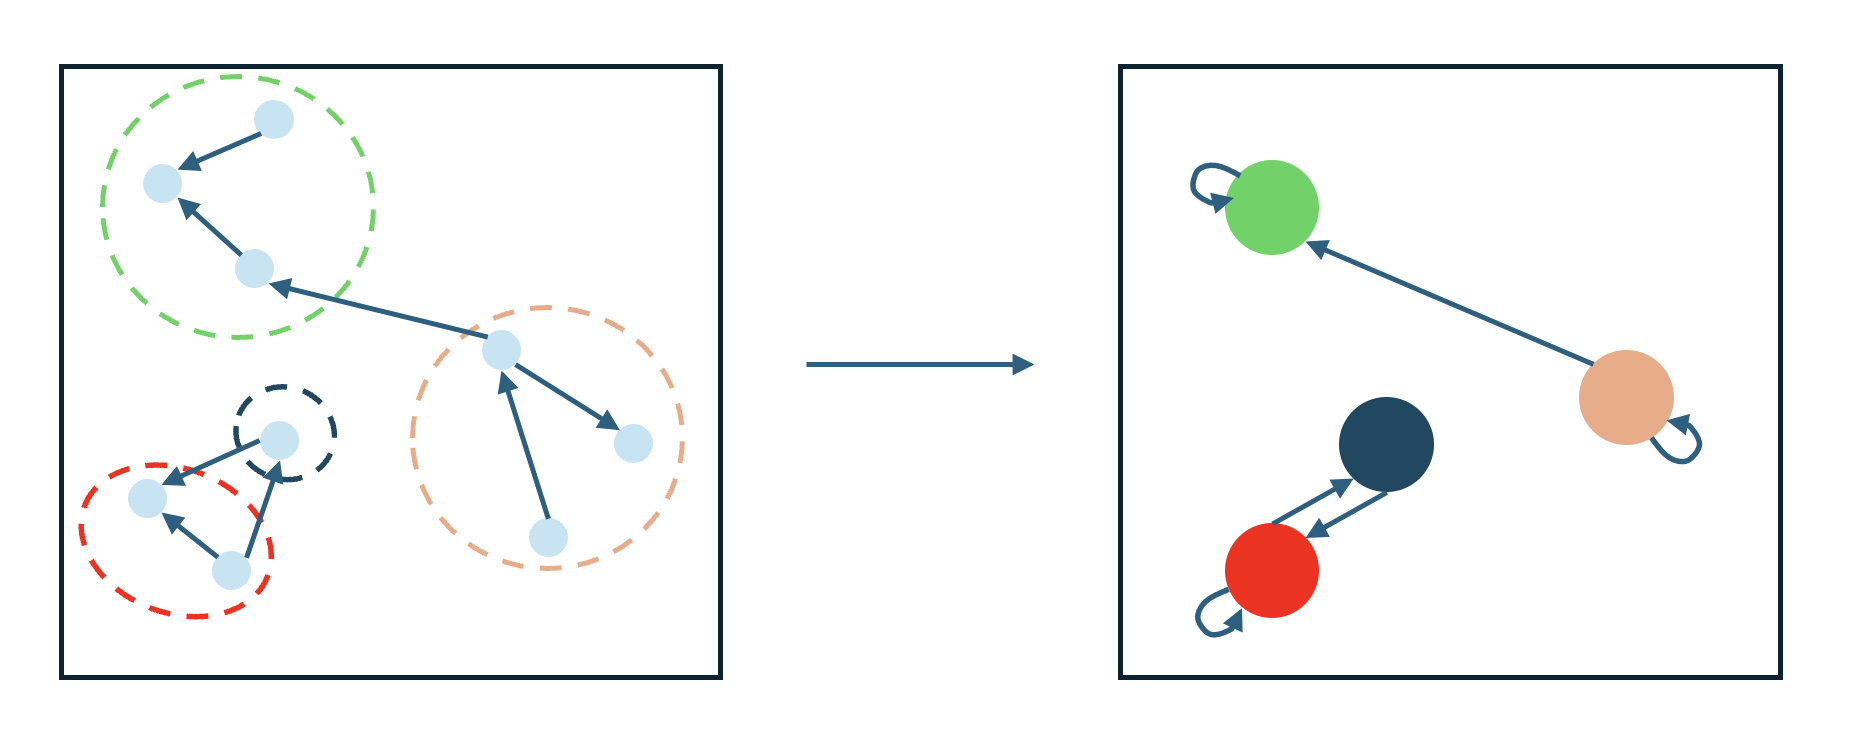
\includegraphics[scale=0.45]{../img/theory/coarse_graining.png}
        \caption{Illustration of one coarse-graining step in the Scale-invariant model. We can form groups of nodes in an arbitrary way. Then groups are connected only if there is any connection between nodes form those groups. If there is a connection between nodes in the same group, self-loop is formed. If there are links in both directions between nodes from two groups, a reciprocated link is formed.}
        \label{fig:coarse_graining}
    \end{figure}

Let us have the adjacency matrix $\mathbb{A}^{(0)}$ of the initial graph with $N_0$ nodes. We denote its elements as $a_{i_0,j_0}^{(0)}$. If there is a link between $i_0$ and $j_0$, then $a_{i_0,j_0}^{(0)} = 1$, otherwise $a_{i_0,j_0}^{(0)} = 0$. Now, if we make the partitioning in $N_1$ groups, the adjacency matrix $\mathbb{A}^{(1)}$ of the new coarse-grained graph will be 
\begin{equation}
    a_{i_1,j_1}^{(1)} = 1 - \prod_{i_0 \in i_1}\prod_{j_0 \in j_1} (1 - a_{i_0,j_0}^{(0)})
\label{eq_coarse_grain}
\end{equation}
where the expression $i_0 \in i_1$ means, that node $i_0$ is contained in the block-node $i_1$. The expression \ref{eq_coarse_grain} corresponds to the requirement, that we do not connect two groups only if there is no connection between any two nodes from the two groups.

We can denote the partitioning of nodes as a function, which assigns every node to its corresponding group, that is $i_1 = \Omega_0(i_0)$. But now, for the new coarse-grained graph, we can find another partitioning, $\Omega_1$ and perform another level of coarse-graining. We obtain the corresponding adjacency matrix $\mathbb{A}^{(2)}$ similarly. In the end, we can make a sequence of partitionings, $\{\Omega_l\}_{l\geq0}$ and find the corresponding sequence of adjacency matrices $\{\mathbb{A}^{(l)}\}_{l\geq0}$. 

Let us make an important remark. The model aims to allow for arbitrary partitioning, therefore it does not rely on any geometrical embedding. That explains the name of the original paper ``Scale-invariance without geometry''. This is also a difference with other proposed renormalization schemes, both in physics, or in network science, which rely heavily on geometry.

\subsubsection{Scale-invariance}
Now we know how to coarse-grain any graph. With that, we would like to find a random graph model, which can generate graphs in a scale-invariant fashion. We explain, what we mean by that, in the following paragraphs.

Let us assume, that the graph at the lowest-level, $\mathbb{A}^{(0)}$ comes from some probability distribution $P_0(\mathbb{A}^{(0)}, \Theta_0)$, where $\Theta_0$ are parameters of the model. We demand a normalization $\sum_{\mathbb{A}^{(0)} \in \mathcal{G}_{N_0}}P_0(\mathbb{A}^{(0)}, \Theta_0) = 1$, where $\mathcal{G}_{N_0}$ denotes all binary undirected graphs with $N_0$ nodes. Now let us fix some partitioning sequence $\{\Omega_l\}_{l\geq0}$. Since we have a probability of each graph $\mathbb{A}^{(0)} \in \mathcal{G}_{N_0}$, what is the probability of the graph $\mathbb{A}^{(1)}$ at the next coarse-graining level? It is just a sum of probabilities of all graphs $\mathbb{A}^{(0)}$, which end up being coarse grained to the graph $\mathbb{A}^{(1)}$, i.e. \begin{equation}
    P_1(\mathbb{A}^{(1)}, \Theta_1) = \sum_{\{\mathbb{A}^{(0)}\} \xrightarrow{\Omega_0} \mathbb{A}^{(1)}} P_0(\mathbb{A}^{(0)}, \Theta_0)
\end{equation}
where the sum goes over all graphs $\mathbb{A}^{(0)}$ projected on $\mathbb{A}^{(1)}$ by the partitioning $\Omega_0$. $\Theta_1$ are some new model parameters. Similarly, we find the probability of a graph in the $l$-th coarse-graining level to be
\begin{equation}
    P_l(\mathbb{A}^{(l)}, \Theta_l) = \sum_{\{\mathbb{A}^{(0)}\} \xrightarrow{\Omega_{l-1}\dots\Omega_0} \mathbb{A}^{(l)}} P_0(\mathbb{A}^{(0)}, \Theta_0)
\end{equation}
where $\Omega_{l-1}\dots\Omega_0$ is just a composition of partitions $\Omega_{0}$,\dots,$\Omega_{l-1}$. 

The requirement of a scale-invariant model means, that if we want to generate graphs in the $l$-th level, we can either first generate them at the 0-th level and then deterministically coarse-grain, or we can generate them directly at the $l$-th level using the same model. That means, the same model should be valid for all coarse-graining levels in its form, where only the parameters of the model and its dimensionality would change. That corresponds to renormalization in physics, where, by changing the scale, we obtain the same functional form of the model, but with renormalized parameters.

The scale-invariance requirement can be therefore written for any $l \in \mathbb{N}$ as
\begin{equation}
    P(\mathbb{A}^{(l)}, \Theta_l) = \sum_{\{\mathbb{A}^{(0)}\} \xrightarrow{\Omega_{l-1}\dots\Omega_0} \mathbb{A}^{(l)}} P(\mathbb{A}^{(0)}, \Theta_0)
\end{equation}
where we dropped the dependence of probability distribution on coarse-graining level $l$, and where the new parameters $\Theta_l$ are obtained only from the parameters $\Omega_0$ and the knowledge of partitionings $\Omega_{0}$,\dots,$\Omega_{l-1}$. This also implies, that we can start from any level in general, not only the 0-th. Therefore, the most general scale-invariance expression for any $l,m\in\mathbb{N}$, $l>m$ reads

\begin{equation}
    P(\mathbb{A}^{(l)}, \Theta_l) = \sum_{\{\mathbb{A}^{(m)}\} \xrightarrow{\Omega_{l-1}\dots\Omega_m} \mathbb{A}^{(l)}} P(\mathbb{A}^{(m)}, \Theta_m)
\label{eq_scale_invariance}
\end{equation}

\subsubsection{Specifying the model}
Now, let us add more requirements to the model. First, we assume, that the edges are \textbf{independent}.  This is a usual setting for random graph models, and it is a crucial simplification. Entries of the adjacency matrix are independent Bernoulli random variables. The probability of link between node $i_l$ and $j_l$ being present is $p_{i_l,j_l}(\Theta_l)$ (we explicitly denote the dependence on $\Theta_l$ and implicitly assume dependence on fitnesses $x_{i_l}, x_{j_l}$ ). In that case, the graph probability factorizes as
\begin{equation}
    P(\mathbb{A}^{(l)}, \Theta_l) = \prod_{i_l=1}^{N_l}\prod_{j_l=1}^{i_l} [p_{i_l,j_l}(\Theta_l)]^{a_{i_l,j_l}^{(l)}}[1 - p_{i_l,j_l}(\Theta_l)]^{1 - a_{i_l,j_l}^{(l)}}
\end{equation}

Next, let us specify the model parameters. First, we assume a global constant $z_l$, which is tuning the overall density at the $l$-th coarse-graining level. Next, let us assign a 'fitness' parameter $x_{i_l}$ to each node $i_l$ in the $l$-th coarse-graining level. These fitness parameters quantify the overall tendency of nodes to connect to other nodes. Then, we can also assign parameters to all possible pairs of nodes, we denote them $\{d_{i_l,j_l}\}_{i_l,j_l=1}^{N_l}$. The final assumption is, that the fitness parameters are node-additive upon coarse-grainings, i.e. $x_{i_{l+1}} = \sum_{i_l \in i_{l+1}} x_{i_l}$ for any coarse-graining level $l$.

\subsubsection{Finding the functional form}
The equation \ref{eq_scale_invariance} with the requirements above is a functional equation where the goal is to find the suitable form of graph probability, or, since the links are independent, the link probability. Let us show the derivation in the case where 
dyadic parameters $\{d_{i_l,j_l}\}_{i_l,j_l=1}^{N_l}$ are not present. 

Let us have two consecutive levels of coarse-graining, $l$ and $l+1$. Scale-invariance demands, that the functional form of link probability is the same at all coarse-graining levels and that only the parameters change by some renormalization rule. Let us assume two distinct blocks $i_{l+1}$, $j_{l+1}$ of nodes at the level $l+1$. We defined our coarse-graining in such way, that these blocks are not connected only if there are no links between any two nodes from these blocks. The probability, that the blocks $i_{l+1}$ and $j_{l+1}$ are not connected is $1 - p_{i_{l+1},j_{l+1}}(z_{l+1})$. This probability depends on the overall density factor $z_{l+1}$ as well as on fitnesses $x_{i_{l+1}}$, $x_{j_{l+1}}$ (we do not denote this dependence and leave it implicit from the subscripts). The links are independent and therefore the probability, that there are no connections between nodes of the two blocks, is equal $\prod_{i_l\in i_{l+1}}\prod_{j_l\in j_{l+1}}[1-p_{i_l,j_l}(z_l)]$. Therefore, the scale-invariance requirement reads
\begin{equation}
    1 - p_{i_{l+1},j_{l+1}}(z_{l+1}) = \prod_{i_l\in i_{l+1}}\prod_{j_l\in j_{l+1}}[1-p_{i_l,j_l}(z_l)]
\end{equation}

Taking logarithm, we obtain
\begin{equation}
    \ln [1 - p_{i_{l+1},j_{l+1}}(z_{l+1})] = \sum_{i_l\in i_{l+1}}\sum_{j_l\in j_{l+1}}[1-p_{i_l,j_l}(z_l)]
\end{equation}

This equation should hold for all pairs from the $l+1$-th coarse-graining level and all possible partitions. The only possible solution is such, that $z_{l+1} = z_l \equiv z$ and
\begin{equation}
     \ln [1 - p_{i_{l+1},j_{l+1}}(z)] = -zg(x_{i_{l+1}})g(x_{j_{l+1}})
     \label{eq_ln_expression}
\end{equation}
where
\begin{equation}
    g(x_{i_{l+1}}) = \sum_{i_l\in i_{l+1}}g(x_{i_l})
\end{equation}
The density parameter $z$ needs to be positive, so that the probability is correctly defined. Function $g$ needs to have same sign for all nodes, and we can therefore choose it to be positive. Also, since we required the fitnesses to be node-additive, and therefore the only possible choice of $g(x)$ is $g(x) = kx$ for some constant $k$. We can then redefine $z \leftarrow k^2 z$ and rewrite \ref{eq_ln_expression} as
\begin{equation}
    \ln [1 - p_{i_{l+1},j_{l+1}}(z)] = -zx_{i_{l+1}}x_{j_{l+1}}
\end{equation}
In the end, for two distinct block-nodes $i_l \neq j_l$, we obtain
\begin{equation}
    p_{i_l,j_l}(z) = 1 - e^{-zx_{i_l}x_{j_l}}, \qquad z, x_{i_l}, x_{j_l} > 0
\end{equation}
In the case, where $i_l = j_l$, one needs to be careful to not double-count the same edges. Then, the derivation (see Appendix 1 in \cite{Garuccio2023}) leads to
\begin{equation}
    p_{i_l,j_l} = 1 - e^{-\frac{z}{2}x_{i_l}^2}, \qquad z, x_{i_l} >0
\end{equation}

Therefore, we obtained the functional form of the link probability from the requirement of scale-invariance. Also, we have a renormalization rule for the density parameter $z_l$, that is $z_l = z_{l+1} \equiv z$, i.e. density parameter remains constant. The renormalization rule for fitnesses was imposed in advance, $x_{i_{l+1}} = \sum_{i_l\in i_{l+1}} x_{i_l}$.

One can also take in the account the dyadic (edge-specific) parameters $\{d_{i_l,j_l}\}_{i_l,j_l=1}^{N_l}$. In that case, we obtain the most general form of the Scale-Invariant Model (SIM) present in \cite{Garuccio2023}
\begin{equation}
    p_{i_l,j_l} = 
    \begin{cases}1 - e^{zx_{i_l}x_{j_l}}f(d_{i_l,j_l}) \quad \text{if} \quad i_l \neq j_l \\
    1 - e^{-\frac{z}{2}x_{i_l}^2}f(d_{i_l,i_l}) \quad \text{if} \quad i_l = j_l \\
    \end{cases}
\end{equation}
where $z>0$, $x_{i_l} \geq 0 \, \forall i_l$ and f is an arbitrary positive function. The renormalization rules for the model parameters are then
\begin{align}
    z_{l+1} &\equiv z_l \equiv z \\
    x_{i_{l+1}} &\equiv \sum_{x_{i_l}\in x_{i_{l+1}}} \\
    f(d_{i_{l+1},j_{l+1}}) &\equiv \frac{\sum_{i_l\in i_{l+1}}\sum_{j_l\in j_{l+1}}x_{i_l}x_{j_l}f(d_{i_l,j_l})}{\sum_{i_l\in i_{l+1}}x_{i_l}\sum_{j_l\in j_{l+1}}x_{j_l}}
\end{align}
Let us point out, that the dependence on the dyadic factors can be eliminated by choosing function $f$ to be a constant function.

\subsubsection{Directed case}
Recently, Lalli and Garlaschelli generalized the Scale-Invariant Model for directed networks (Directed Scale-Invariant Model - DSIM) \cite{Lalli2024}. They tackled the problem, how to reproduce the nontrivial patterns in reciprocity of directed links in real-world network. Reciprocity refers to a non-trivial tendency of nodes to form mutual (reciprocated) connections.

We denote four probabilities for edges between nodes $i_l$ and $j_l$:
\begin{itemize}
    \item $\overset\rightarrow{p_{i_l,j_l}}(\Theta_l)$ for a single directed link from $i_l$ to $j_l$ and no reciprocal link from $j_l$ to $i_l$
    \item $\overset\leftarrow{p_{i_l,j_l}}(\Theta_l)$ for a single directed link from $j_l$ to $i_l$ and no reciprocal link from $i_l$ to $j_l$
    \item $\overset\leftrightarrow{p_{i_l,j_l}}(\Theta_l)$ for a reciprocated link between $i_l$ and $j_l$
    \item $\overset{\not\leftrightarrow}{p_{i_l,j_l}}(\Theta_l)$ for no link between $i_l$ and $j_l$
\end{itemize}
Let us also denote $p_{i_l,j_l}(\Theta_l)$ to be the marginal probability of a link from $i_l$ to $j_l$. The simplest case would be, that we could factorize the four probabilities using the marginal probability, i.e. $\overset\rightarrow{p_{i_l,j_l}}(\Theta_l) = p_{i_l,j_l}(\Theta_l)(1 - p_{j_l,i_l}(\Theta_l))$, $\overset\leftarrow{p_{i_l,j_l}}(\Theta_l) = p_{j_l,i_l}(\Theta_l)(1 - p_{i_l,j_l}(\Theta_l)$ etc. The authors, however, do not assume this, to reproduce non-trivial reciprocity patterns. 

Firstly, every directed graph can be projected to an undirected one (undirected link between two nodes is present if there is a directed link between those two nodes in at least one direction). We demand this undirected projection to follow the undirected SIM. The undirected connection probability between nodes $i_l$ and $j_l$ can be written as 
\begin{align}
    q_{i_l,j_l} = \overset\rightarrow{p_{i_l,j_l}} + \overset\leftarrow{p_{i_l,j_l}} + \overset\leftrightarrow{p_{i_l,j_l}} = 
    \begin{cases}
        1 - e^{-\delta x_{i_l}x_{j_l}f(d_{i_l,j_l})}, \qquad &i_l \neq j_l\\
        1 - e^{-\frac{\delta}{2}x_{i_l}^2f(d_{i_l,i_l}) - \eta w_{i_l}}, \qquad &i_l = j_l
    \end{cases}
\end{align}
Here, compared to the original SIM, the parameter $\eta$ was introduced together with a new node-dependent fitness $w_{i_l}$. This fitness controls separately the tendency of a node to form self-loops, while $\eta$ controls it globally. Similarly to fitnesses $x_{i_l}$, also $w_{i_l}$ is node-additive under coarse-graining. 

Another marginal probability to consider is the overall probability $p_{i_l,j_l}$ to form a directed link from node $i_l$ to $j_l$, regardless of the presence of a link in the opposite direction. By demanding scale-invariance, one can get the expression
\begin{align}
    p_{i_l,j_l} = \begin{cases}
        1 - e^{-\epsilon y_{i_l}z_{j_l}f(d_{i_l,j_l})}, \qquad &i_l \neq j_l\\
        1 - e^{-\frac{\delta}{2}x_{i_l}^2f(d_{i_l,i_l}) - \eta w_{i_l}}, \qquad &i_l = j_l
    \end{cases}
\end{align}
where $\epsilon$ determines the overall density of directed links. Also, two sets of fitness variables were introduced, $\{y_{i_l}\}_{i_l=1}^{N_l}$ and $\{z_{i_l}\}_{i_l=1}^{N_l}$. These are the tendencies of nodes to form out-going and in-going links respectively. They are also node-additive, similarly to SIM. $\epsilon$ remains unchanged under coarse-graining, while $f(d_{i_l,j_l})$ follows the renormalization rule
\begin{equation}
    f(d_{i_{l+1},j_{l+1}}) \equiv \frac{\sum_{i_l\in i_{l+1}}\sum_{j_l\in j_{l+1}}y_{i_l}z_{j_l}f(d_{i_l,j_l})}{\sum_{i_l\in i_{l+1}}y_{i_l}\sum_{j_l\in j_{l+1}}z_{j_l}}
\end{equation}

Since we know that $q_{i_l,j_l} = \overset\rightarrow{p_{i_l,j_l}} + \overset\leftarrow{p_{i_l,j_l}} + \overset\leftrightarrow{p_{i_l,j_l}}$ and $p_{i_l,j_l} = \overset\rightarrow{p_{i_l,j_l}} + \overset\leftrightarrow{p_{i_l,j_l}}$, we can now find all the expressions for $\overset\rightarrow{p_{i_l,j_l}}$, $\overset\leftarrow{p_{i_l,j_l}}$, $\overset\leftrightarrow{p_{i_l,j_l}}$ and $\overset{\not\leftrightarrow}{p_{i_l,j_l}}$. Than one can study, how the local reciprocities $r_{i_l,j_l} = \text{Prob}(i_l \rightarrow j_l|j_l \rightarrow i_l)$, as well as the overall reciprocity $\langle r\rangle$ (fraction of expected value of reciprocated links to expected value of all links) behave. For that, we encourage the reader to find details in \cite{Lalli2024}. 

\section{Network reconstruction problem}
In this section, we will introduce the network reconstruction problem, mainly following the review by Squartini et al. \cite{Squartini2018}
In the network science, the focus was initially on determining the properties of real-world network. Several observations were made:
\begin{itemize}
    \item Power-law degrees: Real-world networks usually have node degrees, which are power-law distributed, there are few hubs with many connections and most of the nodes with little connections.
    \item Small-world effect: Nodes are usually close to each other. That means that if we have two nodes and find the shortest path along edges between them, this path is typically short.
    \item Large clustering: nodes usually form densely connected groups, which are then less connected with each other.
    \item Assortativity: Average nearest neighbor degree is either positively or negatively correlated with the node degree.
\end{itemize}

Based on these properties, scientists were trying to find models which could reproduce them. We saw some of these models in the previous section. In case of many networks, for example financial ones, another problem can arise. The information about networks in question is often not complete. In case of financial networks, the detailed data are usually not disclosed and only some limited information is available. We can think of a network of banks, which lend to each other. Banks do not disclose every single liability, they only have to announce their overall exposure. On the other hand, knowledge of such a network or its properties is of a high importance, for example to determine the level of risk in case of a crisis. Therefore, it is important to find methods which can reproduce networks well enough even with the limited knowledge. 

Let us now specify the problem setting. We are interested in reconstructing a weighted directed network defined by its $N \times N$ weight-matrix $\hat{W}$. Its entries $\hat{w}_{ij}$ are non-negative real-numbers and the corresponding adjacency matrix can be found by setting $\hat{a}_{ij} = 1 \iff w_{ij} > 0$ and $\hat{a}_{ij} = 0 \iff w_{ij} = 0$
The weights are not directly observable, the only information we have are the node strengths: 
\begin{equation}
    \hat{s}_i^{out} = \sum_{j=1}^N \hat{w}_{ij} \qquad \hat{s}_i^{in} = \sum_{j=1}^N \hat{w}_{ji}
    \label{eq_strength_constraint}
\end{equation}
Sometimes, degrees $\hat{k}_i^{in}$, $\hat{k}_i^{out}$ could be also available. The typical example of such network is the already mentioned matrix of interbank exposures, also called \textit{liability matrix}. 
Then the general goal is to find two matrices, $P$ and $W$, whose entries correspond to probabilities $p_{ij}$ that nodes $i$ and $j$ are connected and $w_{ij}$ the estimates of the edge weight, if they are connected. The available data are of the order $O(N)$, but we need to find $2N^2$, numbers, therefore the problem is under-determined, and we need a statistical approach. In what follows, we will explore few important examples of reconstruction methods. Interested reader can find more in \cite{Squartini2018}.

\subsection{The MaxEnt algorithm}
The MaxEnt algorithm prescribes to maximize the following functional
\begin{equation}
    S = -\sum_{i,j=1}^N w_{ij}\ln w_{ij}
    \label{eq_max_ent_entropy}
\end{equation}
That is an entropy where the probability distribution is given by weights $w_{ij}$. Maximizing \ref{eq_max_ent_entropy} given the constraints \ref{eq_strength_constraint}, we obtain
\begin{equation}
    w_{ij}^{ME} = \frac{\hat{s}_i^{out}\hat{s}_j^{in}}{\hat{W}} \qquad \forall i, j
\end{equation}
where $\hat{W} = \sum_{i=1}^N \hat{s}_i^{out} = \sum_{i=1}^N \hat{s}_i^{in}$. This model is also known from economics as \textit{gravity model}.

We can see, that unless some strength is equal zero, all the weights have non-zero values, therefore we get the corresponding adjacency matrix has all entries equal to 1 and the obtained network is fully connected. That is the biggest disadvantage of this approach - we can not reconstruct any topological properties of the network of interest. Real-world networks are usually very sparse, and therefore a fully-connected network can not serve as a good approximation. Also, the MaxEnt algorithm is deterministic - it returns only one possible configuration. However, we ideally want a more robust model, which would generate a whole ensemble.

\subsection{Directed Weighted Configuration Model}
Let us recall, that in the section \ref{sec_max_ent_ensembles}, we found the so called Directed Binary Configuration Model using the ERG approach with the Hamiltonian $H(G) = \sum_{i=1}^N (\alpha_ik_i^{out}(G) + \beta_i k_i^{in}(G))$. This Hamiltonian corresponds to constraining the node degrees. In the Directed Weighted Configuration Model, we constrain the strengths instead:
\begin{equation}
    H(\textbf{W}) = \sum_{i=1}^N (\gamma_i s_i^{out}(\textbf{W}) + \delta_i s_i^{in}(\textbf{W}))
\end{equation}
This Hamiltonian also allows the resulting graph probability distribution to factorize in simple pairwise distributions $q_{ij}^{DWCM}(w)$:
\begin{equation}
    P(\textbf{W}) = \prod_{i=1}^N \prod_{j(\neq i)=1}^N q_{ij}^{DWCM}(w)
    \label{eq_prob_factorization}
\end{equation}
Computing the probability distribution $q_{ij}^{DWCM}(w)$ in the case of non-negative integer values of $w$, one finds the geometric distribution
\begin{equation}
    q_{ij}^{DWCM}(w) = (y_i^{out}y_j^{in})^w(1-y_i^{out}y_j^{in}) 
\end{equation}
using the reparametrization $y_i^{out} = e^{-\gamma_i}$ and $y_i^{in} = e^{-\delta_i}$. Since the distribution is geometric, one can easily find the expected value:
\begin{equation}
    \langle w_{ij}^{DWCM} \rangle = \frac{y_i^{out}y_j^{in}}{1 - y_i^{out}y_j^{in}}
\end{equation}
The probability that nodes $i$ and $j$ are connected is given by the probability that $w > 0$, which is
\begin{equation}
    p_{ij}^{DWCM} = \sum_{w=1}^\infty  q_{ij}^{DWCM}(w) = y_i^{out}y_j^{in}
\end{equation}
How are the corresponding reparametrized Lagrange multipliers found? Since the model comes from the ERG framework, we know from section \ref{sec_max_ent_ensembles} that the maximum-likelihood estimation corresponds to setting the ensemble averages equal to the empirical properties we included in the Hamiltonian, i.e. we want to solve the equation
\begin{align}
     \hat{s}_i^{out} &= \langle s_i^{out} \rangle \equiv \sum_{j(\neq i)} \langle w_{ij}^{DWCM} \rangle \qquad \forall i \\
    \hat{s}_i^{in} &= \langle s_i^{in} \rangle \equiv \sum_{j(\neq i)} \langle w_{ji}^{DWCM} \rangle \qquad \forall i
\end{align}
This model, however, also usually generates very dense networks, since the observed strengths are usually large and the corresponding connection probabilities are close to 1. Therefore, to reproduce network topology as well, we need some improvements. 

\subsection{Directed Enhanced Configuration Model (DECM)}
First attempt can be to take degree sequences directly into account. That can be achieved by the Hamiltonian
\begin{equation}
    H(\textbf{W}) = \sum_{i=1}^N (\alpha_i k_i^{out}(G) + \beta_i k_i^{in}(G) + \gamma_i s_i^{out}(\textbf{W}) + \delta_i s_i^{in}(\textbf{W}))
\end{equation}
The probability distribution factorizes similarly to \ref{eq_prob_factorization}, but this time with the link-weight probability
\begin{align}
    q_ij^{DECM}(w) = \begin{cases}
        1 - p_{ij}^{DECM} \qquad &\text{if } w=0 \\
        p_{ij}^{DECM}(y_i^{out}y_j^{in})^{w-1}(1-y_i^{out}y_j^{in}) &\text{if } w>0
    \end{cases}
\end{align}
and link probability
\begin{equation}
    p_{ij}^{DECM} = \frac{x_i^{out}x_j^{in}y_i^{out}y_j^{in}}{1 + x_i^{out}x_j^{in}y_i^{out}y_j^{in} - y_i^{out}y_j^{in}}
    \label{eq_DECM_weight_prob}
\end{equation}
where $x_i^{out} = e^{-\alpha_i}$, $x_i^{in} = e^{-\beta_i}$, $y_i^{out} = e^{-\gamma_i}$, $y_i^{in} = e^{-\delta_i}$. Since the weight distribution is geometric as well, we can easily evaluate the expected weight
\begin{equation}
    \langle w_{ij}^{DECM} \rangle = \frac{p_{ij}^{DECM}}{1 - y_i^{out}y_j^{in}}
    \label{eq_DECM_average_weight}
\end{equation}
and we can find the corresponding Lagrange multipliers in the similar manner, i.e. setting the ensemble averages of degrees and strengths to the empirically observed values.

The disadvantage of this model is, that we need to know all the degrees of the empirical network, which is, however, usually not the case.

\subsection{Fitness-induced DECM}
One way to deal with the problem of missing degree information, is to use the so-called \textit{fitness ansatz}. It assumes that each node carries an intrinsic value, \textit{fitness}, which regulates its connectivity to other nodes and which is directly connected to the Lagrange multipliers coupled to degrees in the ERG framework. As mentioned in \cite{Squartini2018}, strengths usually serve well as fitnesses, meaning that one could express $x_i^{out} = f(\hat{s}_i^{out})$ and $x_i^{in} = f(\hat{s}_i^{in})$ for some function $f$. In the case of financial systems, it has been shown that the form $x_i^{out} = \sqrt{z}\hat{s}_i^{out}$, $x_i^{in} = \sqrt{z}\hat{s}_i^{in}$ works well enough. 

One could then propose a two-step model:
\begin{enumerate}
    \item First estimate the degrees in the network using the $DBCM$ model and use the fitness ansatz, leading to a link probability
    \begin{equation}
        p_{ij}^{f-DBCM} = \frac{z\hat{s}_i^{out} \hat{s}_j^{in}}{1 + z\hat{s}_i^{out} \hat{s}_j^{in}}
    \end{equation}
    where the parameter $z$ can be found using the knowledge of the total number of links $\hat{L}$ equating it to the ensemble average of the total number of links, or we could use a knowledge of connectivity of some subset of nodes. 
    \item Using the link-probabilities from the first step in the DECM model, i.e. in equations \ref{eq_DECM_weight_prob} and \ref{eq_DECM_average_weight}, we replace $p_{ij}^{DECM}$ with $p_{ij}^{f-DBCM}$
\end{enumerate}
The DECM model can be very accurate, but also very computationally-demanding. 
\subsection{Degree-corrected Gravity Model}
\label{sec_DCGM}
A simpler alternative to the DECM model is the so-called Degree-corrected Gravity Model. Here, we also use the connection-probabilities using the DBCM and the fitness ansatz, but we assign weights using the MaxEnt recipe:
\begin{align}
    w_{ij}^{dcGM} = \begin{cases}
        0 \qquad &\text{with probability } 1 - p_{ij}^{f-DBCM}\\
        \frac{w_{ij}^{ME}}{p_{ij}^{f-DBCM}} &\text{with probability } p_{ij}^{f-DBCM}
    \end{cases}
\end{align}
Using this method, we get that on average the weight in this model correspond to those from the MaxEnt recipe
\begin{equation}
    \langle w_{ij}^{dcGM} \rangle = 0\cdot (1 - p_{ij}^{f-DBCM}) + \frac{w_{ij}^{ME}}{p_{ij}^{f-DBCM}}\cdot p_{ij}^{f-DBCM} = w_{ij}^{ME}
\end{equation} meaning, that we reproduce the node strengths well, but we can also tune the parameter $z$ in $p_{ij}^{f-DBCM}$ to reproduce the network density correctly.

\subsection{Comparison on real-world data}
In 2018, a big comparison of several network reconstruction models was conducted by authors from many different central banks across the world \cite{Anand2018}. The authors have access to datasets of interbank loan networks, which is not the case for most of the researchers. The study was conducted over 25 different financial network datasets.

Seven reconstruction methods were tested, out of which four were deterministic and three generated ensembles. We will not dive deep into the comparison, we will just mention, that the Degree-corrected Gravity Model was found to be the ``clear winner across all measures of interest'' among the probabilistic methods. 